\documentclass[%
	11pt,
	a4paper,
	utf8,
	%twocolumn
		]{article}	

\usepackage{style_packages/podvoyskiy_article_extended}


\begin{document}
\title{Заметки по Анализу временных рядов и сопряженным вопросам}

\author{\itshape Подвойский А.О.}

\date{}
\maketitle

\thispagestyle{fancy}

Здесь приводятся заметки по некоторым вопросам, касающимся машинного обучения, анализа данных, программирования на языках \texttt{Python}, \texttt{R} и прочим сопряженным вопросам так или иначе, затрагивающим работу с временными рядами.


\shorttableofcontents{Краткое содержание}{1}

\tableofcontents

\section{Приемы работы с библиотекой ETNA}

\subsection{Полезные рерсурсы}

Домашняя страница проекта \url{https://github.com/tinkoff-ai/etna}.

\subsection{Установка}

Установить библиотеку можно как обычно с помощью менеджера пакетов \verb|pip|
\begin{lstlisting}[
style = ironpython,
numbers = none
]
pip install etna
\end{lstlisting}

\subsection{Сжатая сводка по библиотеке, рекомендации}

\begin{itemize}
	\item Я выснил у разработчиков библиотеки, что сегменты это просто различные временные ряды одного набора, разделяющие одну и ту же временную ось. То есть, кажется, что сегменты это скорее компоненты (измерения) временного ряда, а значит объект \verb|TSDataset| оперирует многомерными временными рядами. И вроде у этих измерений обязательно должна быть одна и та же временная ось.
	
	\item Перекрестную проверку с расширяющимся окном (или на скользящем окне) в библиотеке ETNA можно выполнить с помощью метода \verb|backtest()|. 
	
	\item Размер тестовой выборки, как правило, определяется \emph{горизонтом прогнозирования} $ h $, а тот в свою очередь определяется бизнес-требованиями. Если, скажем, интересует прогноз на 14 дней вперед, то и тестовая выборка должна включать 14 более поздних наблюдений.
	
	\item Размер тестовой выборки остается постоянным. Это значит, что метрики качества, полученные в результате вычислений прогнозов каждой обученной модели по тестовому набору, будут последовательны и их можно объединять и сравнивать.
	
	\item Размер обучающей выборки не может быть меньше тестовой выборки.
	
	\item Если данные содержат сезонность, обучающая выборка должна содержать не менее двух полных сезонных циклов (правило $ 2 L $, где $ L $ -- количество периодов в полном сезонном цикле, необходимое для инициализации параметров некоторых моделей, например, для вычисления исходного значения тренда в модели тройного экспоненциального сглаживания), учитывая уменьшение длины ряда при выполнении процедур обычного и сезонного дифференциирования.
	
	\item {\color{blue} \underline{Ширина окна} $ w $ для скользящих статистик (и лаговых признаков) должна быть неменьше горизонта прогнозирования, $ w \geqslant h $ (видимо, для того чтобы поймать паттерн соответствующего горизонта, например, недельный). И \underline{порядок лага} $ lag\_ord $ должен быть неменьше горизонта прогнозирования $ lag\_ord \geqslant h $. Так как в противном случае признаки тестового поднабора данных, построенные на лагах с порядком меньшим горизонта прогнозирования, будут использовать значения целевой переменной из тестового поднабора данных (а это утечка)}.
	
	\item Скользящее среднее используется не только для конструирования признаков, но и в качестве прогнозной модели\footnote{Как и фильтр Калмана, и преобразование Фурье} (когда прогноз -- это скользящее среднее $ n $ последних наблюдений), а также для сглаживания выбросов, краткосрочных колебаний и более четкого выделения долгосрочных тенденций в ряде.
\end{itemize}

\subsection{Стратегии прогнозирования}

Выделяют 5 стратегий прогнозирования:
\begin{itemize}
	\item Recursive,
	
	\item Direct,
	
	\item DirRec,
	
	\item MIMO,
	
	\item DIRMO: MIMO + DirRec.
\end{itemize}

ETNA поддерживает первые две стратегии.

\subsubsection{Рекурсивная стратегия (Recursive strategy)}

Рекурсивная стратегия в ETNA реализуется с помощью \verb|AutoregressivePipeline|. Конвейер \verb|AutoRegressivePipeline| итеративно строит прогноз на \verb|step| шагов вперед и после этого использует предсказанные значения для построения признаков для следующих шагов:
\begin{itemize}
	\item Может работать медленно для небольших временных шагов \verb|step|, так как метод требует пересчета признаков $ horizon / step $ раз,
	
	\item Позволяет использовать лаги, порядок которых меньше длины горизонта прогноза,
	
	\item Может быть неточным для длинных горизонтов,
	
	\item Стабилен для незашумленных временных рядов.
\end{itemize}

\begin{lstlisting}[
style = ironpython,
numbers = none
]
from etna.pipeline import AutoRegressivePipeline

model = CatBoostPerSegmentModel()
transforms = [
	LinearTrendTransform(in_column="target"),
	LagTransform(in_column="target", lags=[i for i in range(1, 1 + NUMBER_OF_LAGS)], out_column="target_lag"),
]

autoregressivepipeline = AutoRegressivePipeline(model=model, transforms=transforms, horizon=HORIZON, step=1)
metrics_recursive_df, forecast_recursive_df, _ = autoregressivepipeline.backtest(
	ts=ts, metrics=[SMAPE(), MAE(), MAPE()]
)
autoregressive_pipeline_metrics = metrics_recursive_df.mean()
\end{lstlisting}

\subsubsection{Прямая стратегия (Direct strategy)}

Прямая стратегия в ETNA реализуется с помощью \verb|Pipeline| и \verb|DirectEnsemble|. Эта стратегия предполагает условную независимость прогнозов.

\verb|Pipeline| реализует версию \emph{прямой стратегии}, в которой для предсказания всех точек обучается только одна модель:
\begin{itemize}
	\item {\color{red}\verb|Pipeline| \underline{не допускает} лаги, порядок которых меньше длины горизонта прогнозирования, то есть для \verb|Pipeline| должно быть $ logs\_order \geqslant h $},
	
	\item Это самый эффективный по времени метод: и с точки зрения обучения, и с точки зрения построения прогноза.
\end{itemize}

Как упоминалось выше, мы не можем использовать лаги, порядок которых меньше длины горизонта прогнозирования, поэтому используются лаги с порядком от

\verb|horizon| и до \verb|horizon + number_of_lags|
\begin{lstlisting}[
style = ironpython,
numbers = none
]
from etna.pipeline import Pipeline

model = CatBoostPerSegmentModel()
transforms = [
	LinearTrendTransform(in_column="target"),
	LagTransform(
		in_column="target",
		lags=list(range(  # lags_order >= horizon
			HORIZON,
			HORIZON + NUMBER_OF_LAGS
		)),
		out_column="target_lag"
	),
]

pipeline = Pipeline(model=model, transforms=transforms, horizon=HORIZON)
metrics_pipeline_df, forecast_pipeline_df, _ = pipeline.backtest(ts=ts, metrics=[SMAPE(), MAE(), MAPE()])
pipeline_metrics = metrics_pipeline_df.mean()
\end{lstlisting}

\verb|DirectEnsemble| обучает отдельный конвейер для прогнозирования каждого подсегмента (subsegment):
\begin{itemize}
	\item Этот метод может быть полезен, когда используются различные конвейеры, которые эффективны на разных горизонтах,
	
	\item Вычислительное время увеличивается с ростом числа базовых конвейеров,
	
	\item Прогнозы по этой стратегии могут выглядеть как ломанная кривая, потому что они получены независимыми моделями.
\end{itemize}

\begin{lstlisting}[
style = ironpython,
numbers = none	
]
from etna.ensembles import DirectEnsemble


horizons = [7, 14]

model_1 = CatBoostPerSegmentModel()
transforms_1 = [
	LinearTrendTransform(in_column="target"),
	LagTransform(
		in_column="target", lags=[i for i in range(horizons[0], horizons[0] + NUMBER_OF_LAGS)], out_column="target_lag"
	),
]
pipeline_1 = Pipeline(model=model_1, transforms=transforms_1, horizon=horizons[0])


model_2 = CatBoostPerSegmentModel()
transforms_2 = [
	LinearTrendTransform(in_column="target"),
	LagTransform(
		in_column="target", lags=[i for i in range(horizons[1], horizons[1] + NUMBER_OF_LAGS)], out_column="target_lag"
	),
]

pipeline_2 = Pipeline(model=model_2, transforms=transforms_2, horizon=horizons[1])

ensemble = DirectEnsemble(pipelines=[pipeline_1, pipeline_2])

metrics_ensemble_df, forecast_ensemble_df, _ = ensemble.backtest(ts=ts, metrics=[SMAPE(), MAE(), MAPE()])
ensemble_metrics = metrics_ensemble_df.mean()
\end{lstlisting}

\verb|DirectEnsemble|, описанный выше требует построения отдельного конвейера для каждого временного подсегмента. Этот конвейер часто имеет много общих частей, а отличается лишь в нескольких. Чтобы упростить определение конвейера, можно использовать \verb|assemble_pipelines|, который создает конвейер по следующим правилам:
\begin{itemize}
	\item Входные модели (горизонты) могут быть заданы как одна модель (горизонт) или как последовательность моделей (горизонтов). В первом случае все созданные конвейеры будут иметь входную модель (горизонт), а во втором случае -- $ i $-ый конвейер будет содержать $ i $-ую модель.
	
	\item Преобразования могут быть определены как последовательность преобразований или как последовательнсоть последовательностей преобразований.
\end{itemize}

\begin{lstlisting}[
style = ironpython,
numbers = none
]from etna.pipeline import assemble_pipelines

models = [CatBoostPerSegmentModel(), CatBoostPerSegmentModel()]
transforms = [
	LinearTrendTransform(in_column="target"),  # эта часть применяется и к первому конвейеру, и ко второму
	[
		LagTransform(  # эта часть применяется только к первому конвейеру
			in_column="target",
			lags=[i for i in range(horizons[0], horizons[0] + NUMBER_OF_LAGS)],
			out_column="target_lag",
		),
		LagTransform(  # эта часть применяется только ко второму конвейеру
			in_column="target",
			lags=[i for i in range(horizons[1], horizons[1] + NUMBER_OF_LAGS)],
			out_column="target_lag",
		),
	],
]

pipelines = assemble_pipelines(models=models, transforms=transforms, horizons=horizons)
pipelines
\end{lstlisting}

\subsection{Регрессоры и экзогенные данные}

\emph{Целевой временной ряд} (target time series) -- это временной ряд, который мы пытаемся прогнозировать. Данные, которые помогают строить прогноз для целевого временного ряда, известные в будущем (например, праздники, погода и пр.) в терминологии ETNA называются \emph{регрессорами}. То есть регрессоры -- это временные ряды, которые сами по себе с точки зрения прогноза не интересны, но могут быть полезны при прогнозировании целевого временного ряда (в терминологии Darts такие временные ряды называют \emph{ковариатами}).

Чтобы повысить качество прогноза модели с помощью регрессоров, нужно знать как эти регрессоры влияли на целевой временной ряд в прошлом и значения этих регрессоров в будущем.

Еще в ETNA выделяют \emph{дополнительные данные} (addiitonal data). Это данные, которые мы не знаем заранее, но которые могут пригодится при прогнозировании целевого временного ряда. Для того чтобы в моделях использовать дополнительные данные, их нужно преобразовать в регрессоры.

\begin{lstlisting}[
style = ironpython,
numbers = none
]
from etna.datasets import TSDataset

target_df = pd.read_csv("data/nordic_merch_sales.csv")
regressor_df = pd.read_csv("data/nordics_weather.csv")

target_df = TSDataset.to_dataset(target_df)
regressor_df = TSDataset.to_dataset(regressor_df)

ts = TSDataset(
    df=target_df,  # целевой временной ряд
    freq="D",
    df_exog=regressor_df,  # экзогенные данные
    known_future="all"
)
\end{lstlisting}

Будем использовать простую модель, поддерживающую регрессоры (ковариаты, экзогенные временные ряды)
\begin{lstlisting}[
style = ironpython,
numbers = none
]
from etna.models import LinearPerSegmentModel

HORIZON = 365
model = LinearPerSegmentModel()
\end{lstlisting}

\begin{lstlisting}[
style = ironpython,
numbers = none
]
from etna.transforms import FilterFeaturesTransform

from etna.transforms import MeanTransform  # math
from etna.transforms import DateFlagsTransform, HolidayTransform  # datetime
from etna.transforms import LagTransform  # lags

transforms = [
	LagTransform(
		in_column="target",
		lags=list(range(HORIZON, HORIZON + 28)),
		out_column="target_lag",
	),
	LagTransform(in_column="tavg", lags=list(range(1, 3)), out_column="tavg_lag"),
		MeanTransform(in_column="tavg", window=7, out_column="tavg_mean"),
		MeanTransform(
		in_column="target_lag_365",
		out_column="target_mean",
		window=104,
		seasonality=7,
	),
	DateFlagsTransform(
		day_number_in_week=True,
		day_number_in_month=True,
		is_weekend=True,
		special_days_in_week=[4],
		out_column="date_flag",
	),
	HolidayTransform(iso_code="SWE", out_column="SWE_holidays"),
	HolidayTransform(iso_code="NOR", out_column="NOR_holidays"),
	HolidayTransform(iso_code="FIN", out_column="FIN_holidays"),
	LagTransform(
		in_column="SWE_holidays",
		lags=list(range(2, 6)),
		out_column="SWE_holidays_lag",
	),
	LagTransform(
		in_column="NOR_holidays",
		lags=list(range(2, 6)),
		out_column="NOR_holidays_lag",
	),
	LagTransform(
		in_column="FIN_holidays",
		lags=list(range(2, 6)),
		out_column="FIN_holidays_lag",
	),
	FilterFeaturesTransform(exclude=["precipitation", "snow_depth", "tmin", "tmax"]),
]
\end{lstlisting}

И как обычно
\begin{lstlisting}[
style = ironpython,
numbers = none
]
from etna.pipeline import Pipeline

pipeline = Pipeline(model=model, transforms=transforms, horizon=HORIZON)
\end{lstlisting}

\begin{lstlisting}[
style = ironpython,
numbers = none
]
from etna.metrics import SMAPE

metrics, forecasts, _ = pipeline.backtest(
    ts,
    metrics=[SMAPE()],
    aggregate_metrics=True,
    n_folds=2
)
\end{lstlisting}

\subsection{Пользовательские модели и преобразования}

\begin{lstlisting}[
style = ironpython,
numbers = none
]
import numpy as np
import pandas as pd

from etna.datasets.tsdataset import TSDataset
from etna.transforms import LagTransform
from etna.transforms import SegmentEncoderTransform
from etna.transforms import DateFlagsTransform
from etna.transforms import LinearTrendTransform
from etna.pipeline import Pipeline
from etna.metrics import MAE
from etna.analysis import plot_backtest
\end{lstlisting}

Как обычно преобразуем Pandas'ий кадр данных в специальный объект \verb|TSDataset|
\begin{lstlisting}[
style = ironpython,
numbers = none
]
df = pd.read_csv("data/example_dataset.csv")
df["timestamp"] = pd.to_datetime(df["timestamp"])
df = TSDataset.to_dataset(df)
ts = TSDataset(df, freq="D")
\end{lstlisting}

В ETNA преобразования (transforms) могут изменить значения столбца или добавить новый. Например:
\begin{itemize}
	\item \verb|DateFlagsTransform| -- добавляет столбец с информацией о дате (номер дня, является ли этот день выходным и пр.),
	
	\item \verb|LinearTrendTransform| -- вычитает линейный тренд из ряда.
\end{itemize}
  
\begin{lstlisting}[
style = ironpython,
numbers = none
]
dates = DateFlagsTransform(
    day_number_in_week=True,
    day_number_in_month=False,
    out_column="dateflag"
)
detrend = LinearTrendTransform(in_column="target")  # удаляет линейный тренд!!!

ts.fit_transform([dates, detrend])
# обратить преобразования можно так
ts.inverse_transform([dates, detrend])
\end{lstlisting}

\subsubsection{Per-segment Custom Transform}

Пример пользовательского преобразования
\begin{lstlisting}[
style = ironpython,
numbers = none
]
from etna.transforms.base import OneSegmentTransform

# Class for processing one segment.
class _OneSegmentFloorCeilTransform(OneSegmentTransform):

	# Constructor with the name of the column to which the transformation will be applied.
	def __init__(self, in_column: str, floor: float, ceil: float):
		"""
		Create instance of _OneSegmentLinearTrendBaseTransform.
		
		Parameters
		----------
		in_column:
		name of processed column
		floor:
		lower bound
		ceil:
		upper bound
		"""
		self.in_column = in_column
		self.floor = floor
		self.ceil = ceil

	# Provide the necessary training. For example calculates the coefficients of a linear trend.
	# In this case, we calculate the indices that need to be changed
	# and remember the old values for inverse transform.
	def fit(self, df: pd.DataFrame) -> "_OneSegmentFloorCeilTransform":
		"""
		Calculate the indices that need to be changed.
		
		Returns
		-------
		self
		"""
		target_column = df[self.in_column]
		
		self.floor_indices = target_column < self.floor
		self.floor_values = target_column[self.floor_indices]
		
		self.ceil_indices = target_column > self.ceil
		self.ceil_values = target_column[self.ceil_indices]
		
		return self

	# Apply changes.
	def transform(self, df: pd.DataFrame) -> pd.DataFrame:
		"""
		Drive the value to the interval [floor, ceil].
		
		Parameters
		----------
		df:
		DataFrame to transform
		
		Returns
		-------
		transformed series
		"""
		result_df = df
		result_df[self.in_column].iloc[self.floor_indices] = self.floor
		result_df[self.in_column].iloc[self.ceil_indices] = self.ceil
		
		return result_df

	# Returns back changed values.
	def inverse_transform(self, df: pd.DataFrame) -> pd.DataFrame:
		"""
		Inverse transformation for transform. Return back changed values.
		
		Parameters
		----------
		df:
		data to transform
		
		Returns
		-------
		pd.DataFrame
		reconstructed data
	"""
	result = df
	result[self.in_column][self.floor_indices] = self.floor_values
	result[self.in_column][self.ceil_indices] = self.ceil_values
	
	return result
\end{lstlisting}

Теперь можно определить класс, который будет работать со всем набором данных, применяя преобразование (\verb|_OneSegmentFloorCeilTransform|) к каждому сегменту.

Есть два варианта \verb|PerSegmentWrapper|:
\begin{itemize}
	\item \verb|IrreversiblePerSegmentWrapper| -- базовый класс преобразований по сегментам без обращения преобразований. Этот класс реализует \verb|inverse_transform| просто возвращая весь набор данных.
	
	\item \verb|ReversiblePerSegmentWrapper| -- базовый класс преобразований по сегментам, поддерживающий пользовательские обратные преобразования. Этот класс реализует логику \verb|inverse_transform|, вызывая соответсвующий метод \verb|OneSegmentTransform| для каждого сегмента.
\end{itemize}

В обоих случаях нужно реализовать только метод \verb|get_regressors_info| -- он должен возвращать регрессоры, созданные преобразованием.

\begin{lstlisting}[
style = ironpython,
numbers = none	
]
from etna.transforms.base import ReversiblePerSegmentWrapper
from typing import List

class FloorCeilPerSegmentTransform(ReversiblePerSegmentWrapper):
"""Transform that truncate values to an interval [ceil, floor]"""

	def __init__(self, in_column: str, floor: float, ceil: float):
		"""Create instance of FloorCeilTransform.
		Parameters
		----------
		in_column:
		name of processed column
		floor:
		lower bound
		ceil:
		upper bound
		"""
		self.in_column = in_column
		self.floor = floor
		self.ceil = ceil
		super().__init__(
			transform=_OneSegmentFloorCeilTransform(in_column=self.in_column, floor=self.floor, ceil=self.ceil),
			required_features=[in_column],
		)

	# Here we need to specify output columns with regressors, if transform creates them.
	def get_regressors_info(self) -> List[str]:
		"""Return the list with regressors created by the transform.
		
		Returns
		-------
		:
		List with regressors created by the transform.
		"""
		return []
\end{lstlisting}

\subsubsection{Multi-segment Custom Transform}

Теперь рассмотрим реализацию преобразования для мульти-сегментов. Для мульти-сегментов есть такое же разделение по базовым классам:
\begin{itemize}
	\item \verb|IrreversibleTransform| -- базовый класс для мульти-сегментных преобразований без обратных преобразований. Этот класс реализует \verb|inverse_transform| просто возвращая весь набор данных. Другая логика должна быть реализована с помощью \verb|_fit| и \verb|_transform|.
	
	\item \verb|ReversibleTransform| -- базовый класс для мульти-сегментных преобразований с поддержикой пользовательских обратных преобразований. В дополнение к методам \verb|_fit|, \verb|_transform| здесь следует реализовать логику обращения преобразования в методе \verb|_inverse_transform|. 
\end{itemize}

\begin{lstlisting}[
style = ironpython,
numbers = none
]
from etna.transforms.base import ReversibleTransform


# Class for processing one segment.
class FloorCeilMultiSegmentTransform(ReversibleTransform):

	# Constructor with the name of the column to which the transformation will be applied.
	def __init__(self, in_column: str, floor: float, ceil: float):
		"""
		Create instance of FloorCeilMultiSegmentTransform.
		
		Parameters
		----------
		in_column:
		name of processed column
		floor:
		lower bound
		ceil:
		upper bound
		"""
		super().__init__(required_features=[in_column])  # only these features will be passed to the other methods
		self.in_column = in_column
		self.floor = floor
		self.ceil = ceil

	# Provide the necessary training. For example calculates the coefficients of a linear trend.
	# In this case, we calculate the indices that need to be changed
	# and remember the old values for inverse transform.
	def _fit(self, df: pd.DataFrame) -> "FloorCeilMultiSegmentTransform":
		"""
		Calculate the indices that need to be changed.
		
		Returns
		-------
		self
		"""
		target_column = df.loc[pd.IndexSlice[:], pd.IndexSlice[:, self.in_column]]
		
		self.floor_indices = target_column < self.floor
		self.floor_values = target_column[self.floor_indices]
		
		self.ceil_indices = target_column > self.ceil
		self.ceil_values = target_column[self.ceil_indices]
		
		return self

	# Apply changes.
	def _transform(self, df: pd.DataFrame) -> pd.DataFrame:
		"""
		Drive the value to the interval [floor, ceil].
		
		Parameters
		----------
		df:
		DataFrame to transform
		
		Returns
		-------
		transformed series
		"""
		result_df = df
		result_df[self.floor_indices] = self.floor
		result_df[self.ceil_indices] = self.ceil
		
		return result_df

	# Returns back changed values.
	def _inverse_transform(self, df: pd.DataFrame) -> pd.DataFrame:
		"""
		Inverse transformation for transform. Return back changed values.
		
		Parameters
		----------
		df:
		data to transform
		
		Returns
		-------
		pd.DataFrame
		reconstructed data
		"""
		result_df = df
		result_df[self.floor_indices] = self.floor_values[self.floor_indices]
		result_df[self.ceil_indices] = self.ceil_values[self.ceil_indices]
		
		return result_df

	# Here we need to specify output columns with regressors, if transform creates them.
	def get_regressors_info(self) -> List[str]:
		"""Return the list with regressors created by the transform.
		
		Returns
		-------
		:
		List with regressors created by the transform.
		"""
		return []
\end{lstlisting}

Применяем преобразования
\begin{lstlisting}[
style = ironpython,
numbers = none
]
from copy import deepcopy

bounds_multi_segment = FloorCeilMultiSegmentTransform(in_column="target", floor=150, ceil=600)
bounds_per_segment = FloorCeilPerSegmentTransform(in_column="target", floor=150, ceil=600)

df_per_segment = bounds_per_segment.fit_transform(deepcopy(ts)).to_pandas()
df_multi_segment = bounds_multi_segment.fit_transform(deepcopy(ts)).to_pandas()
pd.testing.assert_frame_equal(df_per_segment, df_multi_segment)
\end{lstlisting}

\subsubsection{Пользовательская модель}

Для того чтобы создать пользовательскую модель с нуля, нужно сначала выбрать базовый класс:
\begin{itemize}
	\item \verb|NonPredictionIntervalContextIgnorantAbstractModel|: модель не может генерировать интервалы прогноза и не требует контекста для построения прогноза,
	
	\item \verb|NonPredictionIntervalContextRequiredAbstractModel|: модель не может генерировать интервалы прогноза и требует контекст для построения прогноза,
	
	\item \verb|PredictionIntervalContextIgnorantAbstractModel|: модель может генерировать интервалы прогноза и не требует контекста для построения прогноза,
	
	\item \verb|PredictionIntervalContextRequiredAbstractModel|: модель может генерировать интервалы прогноза и требует контекст для построения прогноза.
\end{itemize}

Эти классы имеют различные сигнатуры вызова для методов \verb|forecast| и \verb|predict|:
\begin{itemize}
	\item Все сигнатуры принимают \verb|ts: TSDataset| для построения прогноза и \verb|return_components: bool|, который указывает на то, следует проводить декомпозицию или нет.
	
	\item Если модель может генерировать интервалы для прогнозов, то еще нужно передать
	
	 \verb|prediction_interval: bool| и \verb|quantiles: Sequence[float]|,
	
	\item Если модель требует контекст, то еще нужно передать \verb|prediction_size: int|, чтобы отличать контекст от точек, для которых мы строим прогноз.
\end{itemize}

\emph{Контекст} -- это часть набора данных перед точкой прогноза, которые необходимы для построения прогноза. Это требуется для моделей, которые по своей сути используют предыдущие точки для построения прогнозов. Например, \verb|etna.models.NaiveModel(lag=1)|, которая использует последнюю точку для предсказания следующей.

Что же касается модели \verb|LightGBM|, то она не требует контекста
\begin{lstlisting}[
style = ironpython,
numbers = none
]
from lightgbm import LGBMRegressor
from etna.models.base import NonPredictionIntervalContextIgnorantAbstractModel

class LGBMModel(NonPredictionIntervalContextIgnorantAbstractModel):
	def __init__(
		self,
		boosting_type="gbdt",
		num_leaves=31,
		max_depth=-1,
		learning_rate=0.1,
		n_estimators=100,
		**kwargs,
	):
		self.boosting_type = boosting_type
		self.num_leaves = num_leaves
		self.max_depth = max_depth
		self.learning_rate = learning_rate
		self.n_estimators = n_estimators
		self.kwargs = kwargs
		self.model = LGBMRegressor(
			boosting_type=self.boosting_type,
			num_leaves=self.num_leaves,
			max_depth=self.max_depth,
			learning_rate=self.learning_rate,
			n_estimators=self.n_estimators,
			**self.kwargs,
		)

	def fit(self, ts: TSDataset) -> "LGBMModel":
		"""Fit model.
		
		Parameters
		----------
		ts:
		Dataset with features
		
		Returns
		-------
		:
		Model after fit
		"""
		df = ts.to_pandas(flatten=True)
		df = df.dropna()
		features = df.drop(columns=["timestamp", "segment", "target"])
		self._categorical = features.select_dtypes(include=["category"]).columns.to_list()
		target = df["target"]
		self.model.fit(X=features, y=target, categorical_feature=self._categorical)

	def forecast(self, ts: TSDataset, return_components: bool = False) -> TSDataset:
		"""Make predictions.
		Prediction decomposition is based on SHAP values for LGBM.
		
		Parameters
		----------
		ts:
		Dataset with features
		return_components:
		If True additionally returns prediction components
		
		Returns
		-------
		:
		Dataset with predictions
		"""
		horizon = len(ts.df)
		df = ts.to_pandas(flatten=True)
		features = df.drop(columns=["timestamp", "segment", "target"])

		y_flat = self.model.predict(features)
		
		y = y_flat.reshape(-1, horizon).T
		ts.loc[:, pd.IndexSlice[:, "target"]] = y
		
		if return_components:
		ts = self.forecast_components(ts=ts)
		
		return ts

	def forecast_components(self, ts: TSDataset) -> TSDataset:
		"""Estimate prediction decomposition using SHAP values.
		
		Parameters
		----------
		ts:
		Dataset with features
		
		Returns
		-------
		:
		Dataset with predictions
		"""
		df = ts.to_pandas(flatten=True)
		features = df.drop(columns=["timestamp", "segment", "target"])
		
		# estimate SHAP values for prediction decomposition
		shap_values = self.model.predict(features, pred_contrib=True)
		
		# encapsulate expected contribution into components
		components = shap_values[:, :-1] + shap_values[:, -1, np.newaxis] / (shap_values.shape[1] - 1)
		
		# components names should start with prefix `target_component_`
		component_names = [f"target_component_{name}" for name in features.columns]
		
		components_df = pd.DataFrame(data=components, columns=component_names)
		components_df["timestamp"] = df["timestamp"]
		components_df["segment"] = df["segment"]
		components_df = TSDataset.to_dataset(df=components_df)

		# adding estimated components to dataset with predictions
		ts.add_target_components(target_components_df=components_df)
		
		return ts

	def predict(self, ts: TSDataset, return_components: bool = False) -> TSDataset:
		"""Make predictions.
		
		Parameters
		----------
		ts:
		Dataset with features
		return_components:
		If True additionally returns prediction components
		
		Returns
		-------
		:
		Dataset with predictions
		"""
		return self.forecast(ts=ts, return_components=return_components)

	def get_model(self) -> LGBMRegressor:
		"""Get internal lightgbm model.
		
		Returns
		-------
		:
		lightgbm model.
		"""
		return self.model
\end{lstlisting}

\begin{lstlisting}[
style = ironpython,
numbers = none
]
HORIZON = 31

trend = LinearTrendTransform(in_column="target")
lags = LagTransform(in_column="target", lags=list(range(31, 96, 1)), out_column="lag")
date_flags = DateFlagsTransform(
	day_number_in_week=True,
	day_number_in_month=True,
	week_number_in_month=True,
	week_number_in_year=True,
	month_number_in_year=True,
	year_number=True,
	special_days_in_week=[5, 6],
	out_column="dateflag",
)
segment_encoder = SegmentEncoderTransform()

transforms = [
	trend,
	lags,
	date_flags,
	segment_encoder,
]
\end{lstlisting}

\begin{lstlisting}[
style = ironpython,
numbers = none
]
model = LGBMModel(random_state=42)
pipeline = Pipeline(model=model, transforms=transforms, horizon=HORIZON)
metrics_df, forecast_df, _ = pipeline.backtest(ts=ts, metrics=[MAE()], n_folds=3)
\end{lstlisting}

\begin{lstlisting}[
style = ironpython,
numbers = none
]
trend = LinearTrendTransform(in_column="target")
lags = LagTransform(in_column="target", lags=list(range(31, 96, 1)), out_column="lag")
date_flags = DateFlagsTransform(
	day_number_in_week=True,
	day_number_in_month=True,
	week_number_in_month=True,
	week_number_in_year=True,
	month_number_in_year=True,
	year_number=True,
	special_days_in_week=[5, 6],
	out_column="dateflag",
)
segment_encoder = SegmentEncoderTransform()

transforms = [
	trend,
	lags,
	date_flags,
	segment_encoder,
]
\end{lstlisting}

\begin{lstlisting}[
style = ironpython,
numbers = none
]
model = LGBMModel(random_state=42)
pipeline = Pipeline(model=model, transforms=transforms, horizon=HORIZON)
metrics_df, forecast_df, _ = pipeline.backtest(ts=ts, metrics=[MAE()], n_folds=3)
\end{lstlisting}

\subsubsection{Создание новой модели с помощью интерфейса Sklearn}

Создадим модель с помощью готовых классов:
\begin{itemize}
	\item \verb|etna.models.SklearnPerSegmentModel|,
	
	\item \verb|etna.models.SklearnMultiSegmentModel|.
\end{itemize}

Сначала реализуем ETNA-модель для каждого сегмента
\begin{lstlisting}[
style = ironpython,
numbers = none
]
from etna.models import SklearnPerSegmentModel
from etna.models import SklearnMultiSegmentModel

class LGBMPerSegmentModel(SklearnPerSegmentModel):
	def __init__(
		self,
		boosting_type="gbdt",
		num_leaves=31,
		max_depth=-1,
		learning_rate=0.1,
		n_estimators=100,
		**kwargs,
	):
	self.boosting_type = boosting_type
	self.num_leaves = num_leaves
	self.max_depth = max_depth
	self.learning_rate = learning_rate
	self.n_estimators = n_estimators
	self.kwargs = kwargs
	model = LGBMRegressor(
		boosting_type=self.boosting_type,
		num_leaves=self.num_leaves,
		max_depth=self.max_depth,
		learning_rate=self.learning_rate,
		n_estimators=self.n_estimators,
		**self.kwargs,
	)
	super().__init__(regressor=model)


class LGBMMultiSegmentModel(SklearnMultiSegmentModel):
	def __init__(
		self,
		boosting_type="gbdt",
		num_leaves=31,
		max_depth=-1,
		learning_rate=0.1,
		n_estimators=100,
		**kwargs,
	):
	self.boosting_type = boosting_type
	self.num_leaves = num_leaves
	self.max_depth = max_depth
	self.learning_rate = learning_rate
	self.n_estimators = n_estimators
	self.kwargs = kwargs
	model = LGBMRegressor(
		boosting_type=self.boosting_type,
		num_leaves=self.num_leaves,
		max_depth=self.max_depth,
		learning_rate=self.learning_rate,
		n_estimators=self.n_estimators,
		**self.kwargs,
	)
	super().__init__(regressor=model)
\end{lstlisting}

\begin{lstlisting}[
style = ironpython,
numbers = none
]
model = LGBMMultiSegmentModel(random_state=42)
pipeline = Pipeline(model=model, transforms=transforms, horizon=HORIZON)
metrics_df_multi_segment, forecast_df, _ = pipeline.backtest(ts=ts, metrics=[MAE()], n_folds=3)
\end{lstlisting}

Если требуется организовать специальную обработку категориальных признаков, то можно написать свою собственную реализацию, взяв за основу \verb|etna.models.CatBoostPerSegmentModel| или \verb|etna.models.CatBoostMultiSegmentModel|





\subsection{Примеры использования}

\subsubsection{Начало}

Кадр данных, представляющих временной ряд должен содержать следующие столбцы:
\begin{itemize}
	\item \verb|target|: столбец, который нужно предсказывать,
	
	\item \verb|timestamp|: столбец с временными метками,
	
	\item \verb|segment|: имя сегмента, так как в общем случае ETNA ориентируется на многомерные временные ряды. В случае одномерного ряда получается такой вот атрибут-артефакт.
\end{itemize}

\begin{lstlisting}[
style = ironpython,
numbers = none	
]
import pandas as pd

original_df = pd.read_csv("data/monthly-australian-wine-sales.csv")
# month -> timestamp, sales -> target
original_df["timestamp"] = pd.to_datetime(original_df["month"])
original_df["target"] = original_df["sales"]
original_df.drop(columns=["month", "sales"], inplace=True)
original_df["segment"] = "main"
\end{lstlisting}

Библиотека ETNA работает со специальной структурой данных \verb|TSDataset|, поэтому сначала классический \verb|DataFrame| преобразовать в \verb|TSDataset|
\begin{lstlisting}[
style = ironpython,
numbers = none
]
from etna.datasets.tsdataset import TSDataset

original_df: pd.DataFrame
df: pd.DataFrame = TSDdataset.to_dataset(original_df)
\end{lstlisting}

А вот теперь можно построить \verb|TSDataset|
\begin{lstlisting}[
style = ironpython,
numbers = none
]
ts: TSDataset = TSDataset(df, freq="MS")
\end{lstlisting}

Можно посмотреть базовую инфомрацию
\begin{lstlisting}[
style = ironpython,
numbers = none
]
ts.info()
"""
<class 'etna.datasets.TSDataset'>
num_segments: 1
num_exogs: 0
num_regressors: 0
num_known_future: 0
freq: MS
start_timestamp end_timestamp  length  num_missing
segments                                                   
main          1980-01-01    1994-08-01     176            0
"""
\end{lstlisting}

Или в формате кадра данных
\begin{lstlisting}[
style = ironpython,
numbers = none
]
ts.describe()
\end{lstlisting}

Построим прогноз с помощью простой модели \verb|NaivModel|
\begin{lstlisting}[
style = ironpython,
numbers = none
]
train_ts, test_ts = ts.train_test_split(
    train_start="1980-01-01",
    train_end="1993-12-01",
    test_start="1994-01-01",
    test_end="1994-08-01",
)
\end{lstlisting}

\begin{lstlisting}[
style = ironpython,
numbers = none	
]
from etna.models import NaiveModel
HORIZON = 8

# Fit the model
model = NaiveModel(lag=12)
model.fit(train_ts)

# Make the forecast
future_ts = train_ts.make_future(
    future_steps=HORIZON,
    tail_steps=model.context_size
)
forecast_ts = model.forecast(
    future_ts,
    prediction_size=HORIZON
)
\end{lstlisting}

Оценим качество прогноза
\begin{lstlisting}[
style = ironpython,
numbers = none
]
from etna.metrics import SMAPE

smape = SMAPE()
smape(y_true=test_ts, y_pred=forecast_ts)  # {'main': 11.492045838249387}
\end{lstlisting}

Теперь построим прогноз с помощью Catboost
\begin{lstlisting}[
style = ironpython,
numbers = none
]
from etna.transforms import LagTransform, LogTransform

lags = LagTransform(
    in_column="target",
    lags=list(rante(8, 24, 1))
)
log = LogTransform(in_column="target")
transforms = [log, lags]
# Преобразования применяются к обчающему фрагменту ряда на месте
train_ts.fit_transform(transforms)
\end{lstlisting}

\begin{lstlisting}[
style = ironpython,
numbers = none
]
from etna.models import CatBoostMultiSegmentModel

model = CatBoostMultiSegmentModel()
model.fit(train_ts)
future_ts = train_ts.make_future(future_steps=HORIZON, transforms=transforms)
forecast_ts = model.forecast(future_ts)
forecast_ts.inverse_transform(transforms)
\end{lstlisting}

\begin{lstlisting}[
style = ironpython,
numbers = none
]
from etna.metrics import SMAPE

smape = SMAPE()
smape(y_true=test_ts, y_pred=forecast_ts)  # {'main': 10.657026308972483}
\end{lstlisting}

Все шаги можно собрать в конвейер
\begin{lstlisting}[
style = ironpython,
numbers = none	
]
from etna.pipeline import Pipeline

train_ts, test_ts = ts.train_test_split(
	train_start="2019-01-01",
	train_end="2019-10-31",
	test_start="2019-11-01",
	test_end="2019-11-30",
)

model = Pipeline(
	model=CatBoostMultiSegmentModel(),
	transforms=transforms,
	horizon=HORIZON,
)
model.fit(train_ts)
forecast_ts = model.forecast()

smape = SMAPE()
smape(y_true=test_ts, y_pred=forecast_ts)
\end{lstlisting}

\subsubsection{Обратное тестирование. Backtest}

\begin{lstlisting}[
style = ironpython,
numbers = none
]
import pandas as pd
import matplotlib.pyplot as plt

from etna.datasets.tsdataset import TSDataset
from etna.metrics import MAE
from etna.metrics import MSE
from etna.metrics import SMAPE
from etna.pipeline import Pipeline
from etna.models import ProphetModel
from etna.analysis import plot_backtest
\end{lstlisting}

Пример обратного тестирования на 3-х фолдах (\pic{fig:backtest}).

\begin{figure}[h]
	\centering
	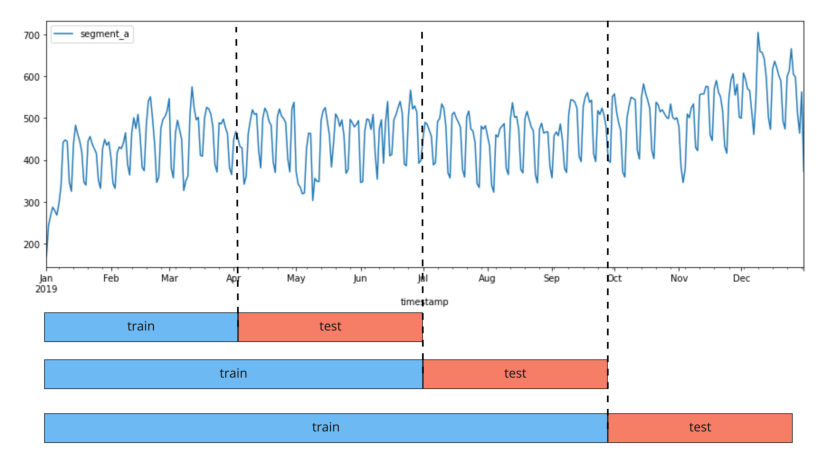
\includegraphics[scale=1.0]{figures/backtest.png}
	\caption{ Обратное тестирование на 3-х фолдах }\label{fig:backtest}
\end{figure}

\begin{lstlisting}[
style = ironpython,
numbers = none
]
df = pd.read_csv("./data/example_dataset.csv")
df = TSDataset.to_dataset(df)
ts = TSDataset(df, freq="D")
\end{lstlisting}

Создадим цепочку преобразований
\begin{lstlisting}[
style = ironpython,
numbers = none
]
horizon = 31  # Set the horizon for predictions
model = ProphetModel()  # Create a model
transforms = []  # A list of transforms -  we will not use any of them

pipeline = Pipeline(model=model, transforms=transforms, horizon=horizon)
\end{lstlisting}

Метод \verb|backtest()| возвращает три кадра данных:
\begin{itemize}
	\item кадр данных с метриками для каждого фолда и каждого сегмента,
	
	\item кадр данных с прогнозами,
	
	\item кадр данных с информацией по каждому фолду.
\end{itemize}

\begin{lstlisting}[
style = ironpython,
numbers = none
]
metrics_df, forecast_df, fold_info_df = pipeline.backtest(
    ts=ts,
    metrics=[
        MAE(),
        MSE(),
        SMAPE(),
    ]
)
\end{lstlisting}

Можно получить метрики, усредненные по фолдам
\begin{lstlisting}[
style = ironpython,
numbers = none
]
metrics_df, forecast_df, fold_info_df = pipeline.backtest(
    ts=ts,
    metrics=[
        MAE(),
        MSE(),
        SMAPE()
    ],
    aggregate_metrics=True,
)
\end{lstlisting}

Обратное тестирование с масками для фолдов. Рассмотрим 3 стратегии: \verb|SlidingWindowSplitter|, \verb|ExpandingWindowSplitter| и \verb|SingleWindowSplitter| (из \verb|sktime|).

Чтобы использовать стратегию расширяющегося окна \verb|ExpandingWindowSplitter|, достаточно просто использовать \verb|mode="expand"|
\begin{lstlisting}[
style = ironpython,
numbers = none
]
metrics_df, _, _ = pipeline.backtest(
    ts=ts,
    metrics=[
        MAE(),
        MSE(),
        SMAPE()
    ],
    n_folds=3,
    mode="expand"
)
\end{lstlisting}

Для того чтобы использовать стратегию \verb|SlidingWindowSplitter|
\begin{lstlisting}[
style = ironpython,
numbers = none
]
from etna.pipeline import FoldMask
import numpy as np

# 1 Without mask
metrics_df, _, _ = pipeline.backtest(
    ts=ts,
    metrics=[
        MAE(),
        MSE(),
        SMAPE()
    ],
    n_folds=1
)
\end{lstlisting}

Или с маской
\begin{lstlisting}[
style = ironpython,
numbers = none
]
# 2 With specific mask
window_size = 85
first_train_timestamp = ts.index.min() + np.timedelta64(100, "D")
last_train_timestamp = first_train_timestamp + np.timedelta64(window_size, "D")
target_timestamps = pd.date_range(start=last_train_timestamp + np.timedelta64(1, "D"), periods=horizon)
mask = FoldMask(
	first_train_timestamp=first_train_timestamp,
	last_train_timestamp=last_train_timestamp,
	target_timestamps=target_timestamps,
)

metrics_df, _, _ = pipeline.backtest(ts=ts, metrics=[MAE(), MSE(), SMAPE()], n_folds=[mask])
\end{lstlisting}

Чтобы использовать стратегию скользящего окна \verb|SlidingWindowSplitter|, нужно создать список масок для фолдов \verb|FoldMask|
\begin{lstlisting}[
style = ironpython,
numbers = none
]
n_folds = 3

def sliding_window_masks(window_size, n_folds):
	masks = []
	for n in range(n_folds):
		first_train_timestamp = ts.index.min() + np.timedelta64(100, "D") + np.timedelta64(n, "D")
		last_train_timestamp = first_train_timestamp + np.timedelta64(window_size, "D")
		target_timestamps = pd.date_range(start=last_train_timestamp + np.timedelta64(1, "D"), periods=horizon)
		mask = FoldMask(
			first_train_timestamp=first_train_timestamp,
			last_train_timestamp=last_train_timestamp,
			target_timestamps=target_timestamps,
		)
		masks.append(mask)
		return masks
\end{lstlisting}

\begin{lstlisting}[
style = ironpython,
numbers = none
]
masks = sliding_window_masks(window_size=window_size, n_folds=n_folds)
metrics_df, _, _ = pipeline.backtest(ts=ts, metrics=[MAE(), MSE(), SMAPE()], n_folds=masks)
\end{lstlisting}

\subsubsection{Обнаружение выбросов}

\begin{lstlisting}[
style = ironpython,
numbers = none
]
import pandas as pd
from etna.datasets.tsdataset import TSDataset

classic_df = pd.read_csv("data/example_dataset.csv")
df = TSDataset.to_dataset(classic_df)
ts = TSDataset(df, freq="D")
\end{lstlisting}

\paragraph{Точечные выборосы (Point outliers)}

\emph{Точечные выбросы} (point outliers) -- это отдельные точечные всплески на графике.

\begin{lstlisting}[
style = ironpython,
numbers = none
]
from etna.analysis import (
	get_anomalies_median,
	get_anomalies_density,
	get_anomalies_prediction_interval,
	get_anomalies_hist,
)
from etna.analysis import plot_anomalies
\end{lstlisting}

Можно задать атрибут-столбец, в котором требуется найти аномалии с помощью аргумента \verb|in_column|.

ETNA поддерживает следующие методы обнаружения выбросов:
\begin{itemize}
	\item Метод медианы,
	
	\item Метод плотности,
	
	\item Метод интервалов (только для \verb|ProphetModel| и \verb|SARIMAXModel|),
	
	\item Метод гистограммы (очень медленный).
\end{itemize}

\emph{Метод медиан} (median method)
\begin{lstlisting}[
style = ironpython,
numbers = none
]
anomaly_dict = get_anomalies_median(ts, window_size=100)
"""
{
	'segment_a': [
	    numpy.datetime64('2019-01-01T00:00:00.000000000')
	],
	'segment_b': [],
	'segment_c': [
	    numpy.datetime64('2019-01-23T00:00:00.000000000'),
	    numpy.datetime64('2019-01-31T00:00:00.000000000'),
	    numpy.datetime64('2019-07-01T00:00:00.000000000')
	],
	'segment_d': [
	    numpy.datetime64('2019-01-01T00:00:00.000000000'),
	    numpy.datetime64('2019-03-12T00:00:00.000000000')
	]
}
"""
plot_anomalies(ts, anomaly_dict)
\end{lstlisting}

\emph{Метод плотности} (density method)
\begin{lstlisting}[
style = ironpython,
numbers = none
]
anomaly_dict = get_anomalies_density(ts, window_size=18, distance_coef=1, n_neighbors=4)
"""
{
	'segment_a': [
	    numpy.datetime64('2019-01-01T00:00:00.000000000'),
	    numpy.datetime64('2019-11-03T00:00:00.000000000')
	],
	'segment_b': [
	    numpy.datetime64('2019-01-01T00:00:00.000000000')
	],
	'segment_c': [
	    numpy.datetime64('2019-01-23T00:00:00.000000000'),
	    numpy.datetime64('2019-05-21T00:00:00.000000000'),
	    numpy.datetime64('2019-07-01T00:00:00.000000000')
	],
	'segment_d': [
	    numpy.datetime64('2019-03-12T00:00:00.000000000')
	]
}
"""
plot_anomalies(ts, anomaly_dict)
\end{lstlisting}

\emph{Метод интервального прогнозирования}. Здесь выбросы -- это точки вне интервала прогнозирования, предсказанного с помощью модели \verb|model|. Сейчас поддерживаются только \verb|ProphetModel| и \verb|SARIMAXModel|
\begin{lstlisting}[
style = ironpython,
numbers = none
]
from etna.models import ProphetModel

anomaly_dict = get_anomalies_prediction_interval(ts, model=ProphetModel, interval_width=0.95)
"""
{
	'segment_a': [
		numpy.datetime64('2019-01-01T00:00:00.000000000'),
		numpy.datetime64('2019-01-02T00:00:00.000000000'),
		numpy.datetime64('2019-01-03T00:00:00.000000000'),
		numpy.datetime64('2019-01-04T00:00:00.000000000'),
		numpy.datetime64('2019-01-07T00:00:00.000000000'),
		numpy.datetime64('2019-01-08T00:00:00.000000000'),
		numpy.datetime64('2019-02-20T00:00:00.000000000'),
		numpy.datetime64('2019-03-01T00:00:00.000000000'),
		numpy.datetime64('2019-03-08T00:00:00.000000000'),
		numpy.datetime64('2019-03-12T00:00:00.000000000'),
		numpy.datetime64('2019-05-01T00:00:00.000000000'),
		numpy.datetime64('2019-05-02T00:00:00.000000000'),
		numpy.datetime64('2019-05-03T00:00:00.000000000'),
		numpy.datetime64('2019-05-09T00:00:00.000000000'),
		numpy.datetime64('2019-05-10T00:00:00.000000000'),
		numpy.datetime64('2019-06-12T00:00:00.000000000'),
		numpy.datetime64('2019-10-27T00:00:00.000000000'),
		numpy.datetime64('2019-11-04T00:00:00.000000000')
	],
	'segment_b': [
		numpy.datetime64('2019-01-01T00:00:00.000000000'),
		numpy.datetime64('2019-01-02T00:00:00.000000000'),
		numpy.datetime64('2019-01-03T00:00:00.000000000'),
		numpy.datetime64('2019-01-07T00:00:00.000000000'),
		numpy.datetime64('2019-01-08T00:00:00.000000000'),
		numpy.datetime64('2019-03-08T00:00:00.000000000'),
		numpy.datetime64('2019-03-12T00:00:00.000000000'),
		numpy.datetime64('2019-05-01T00:00:00.000000000'),
		numpy.datetime64('2019-05-02T00:00:00.000000000'),
		numpy.datetime64('2019-05-03T00:00:00.000000000'),
		numpy.datetime64('2019-05-09T00:00:00.000000000'),
		numpy.datetime64('2019-05-10T00:00:00.000000000'),
		numpy.datetime64('2019-06-12T00:00:00.000000000'),
		numpy.datetime64('2019-06-20T00:00:00.000000000'),
		numpy.datetime64('2019-06-25T00:00:00.000000000'),
		numpy.datetime64('2019-06-27T00:00:00.000000000'),
		numpy.datetime64('2019-11-04T00:00:00.000000000'),
		numpy.datetime64('2019-11-15T00:00:00.000000000')
	],
	'segment_c': [
		numpy.datetime64('2019-05-21T00:00:00.000000000'),
		numpy.datetime64('2019-07-01T00:00:00.000000000')
    ],
	'segment_d': [
		numpy.datetime64('2019-01-01T00:00:00.000000000'),
		numpy.datetime64('2019-01-02T00:00:00.000000000'),
		numpy.datetime64('2019-01-07T00:00:00.000000000'),
		numpy.datetime64('2019-03-08T00:00:00.000000000'),
		numpy.datetime64('2019-03-12T00:00:00.000000000'),
		numpy.datetime64('2019-05-01T00:00:00.000000000'),
		numpy.datetime64('2019-05-02T00:00:00.000000000'),
		numpy.datetime64('2019-05-03T00:00:00.000000000'),
		numpy.datetime64('2019-05-09T00:00:00.000000000'),
		numpy.datetime64('2019-05-10T00:00:00.000000000'),
		numpy.datetime64('2019-06-08T00:00:00.000000000'),
		numpy.datetime64('2019-06-12T00:00:00.000000000'),
		numpy.datetime64('2019-06-16T00:00:00.000000000'),
		numpy.datetime64('2019-06-28T00:00:00.000000000'),
		numpy.datetime64('2019-09-20T00:00:00.000000000'),
		numpy.datetime64('2019-09-30T00:00:00.000000000'),
		numpy.datetime64('2019-10-01T00:00:00.000000000'),
		numpy.datetime64('2019-10-02T00:00:00.000000000'),
		numpy.datetime64('2019-11-04T00:00:00.000000000')
    ]
}
"""
plot_anomalies(ts, anomaly_dict)
\end{lstlisting}

\emph{Гистограммный метод} (histogram method). Здесь выбросы -- это точки, удаление которых из временного ряда, дает гистограмму с меньшей ошибкой аппроксиации. {\color{red}К сожалению, может работать очень медленно.}

Заполнение выбросов можно организовать следующим образом
\begin{lstlisting}[
style = ironpython,
numbers = none
]
from etna.transforms import MedianOutliersTransform, TimeSeriesImputerTransform

df: pd.DataFrame = ts[:, "segment_a", :]  # или так ts.loc[:, ("segment_a", "target")]
ts: TSDataset = TSDataset(df, freq="D")
\end{lstlisting}

Заполнение выбросы выполняется в два этапа:
\begin{itemize}
	\item заменить выбросы, обнаруженные с помощью указанного метода \verb|XxxOutliersTransform|, значениям NaNs,
	
	\item Заполнить значения NaNs с помощью \verb|TimeSeriesImputerTransform|.
\end{itemize}

\begin{lstlisting}[
style = ironpython,
numbers = none
]
best_params = {"window_size": 60, "alpha": 2.35}
outliers_remover = MedianOutliersTransform(in_column="target", **best_params)
ts.fit_transform([outliers_remover])
\end{lstlisting}

Теперь можно заполнить выбросы, обнаруженные методом медианы с помощью стратегии \verb|"running_mean"|
\begin{lstlisting}[
style = ironpython,
numbers = none
]
# Impute NaNs using the specified strategy
outliers_imputer = TimeSeriesImputerTransform(
    in_column="target",
    strategy="running_mean",
    window=30
)

ts.fit_transform([outliers_imputer])
\end{lstlisting}

ВАЖНО! Точки, которые были определены как выбросы могут оказаться точками сложного поведения временных рядов. И тогда их удаление может снизить качество модели.








\listoffigures\addcontentsline{toc}{section}{Список иллюстраций}

% Источники в "Газовой промышленности" нумеруются по мере упоминания 
\begin{thebibliography}{99}\addcontentsline{toc}{section}{Список литературы}
	\bibitem{lutz:learningpython-2011}{\emph{Лутц М.} Изучаем Python, 4-е издание. -- Пер. с англ. -- СПб.: Символ-Плюс, 2011. -- 1280~с. }
	
	\bibitem{geron:hands_on_ml}{\emph{Жерон О.} Прикладное машинное обучение с помощью Scikit-Learn и TensorFlow: концепции, инструменты и техники ля создания интеллектуальных систем. -- СПб.: ООО <<Альфа-книга>>, 2018. -- 688 с.}
	
	\bibitem{burkov:2020}{\emph{Бурков А.} Машинное обучение без лишних слов. -- СПб.: Питер, 2020. -- 192 с.}
	
	\bibitem{burkov-engineer:2022}{\emph{Бурков А.} Инженерия машинного обучения. -- М.:ДМК Пресс, 2022. -- 306 с.}
	
	\bibitem{lakshmanan-mldp:2022}{\emph{Лакшманан В.} Машинное обучение. Паттерны проектирования. -- СПб.: БХВ-Перетбург, 2022. -- 448 с.}
		
	\bibitem{beazley:python-2010}{\emph{Бизли Д.} Python. Подробный справочник. -- Пер. с англ. -- СПб.: Символ-Плюс, 2010. -- 864~с. }
	
	\bibitem{dart:2015}{\emph{Rashmi K.V.}, \emph{Gilad-Bachrach R.} DART: Dropouts meet Multiple Additive Regression Trees, 2015}
	
	\bibitem{ke-lightgbm:2017}{\emph{Ke G. etc.} LightGBM: A Highly Efficient Gradient Boosting Decision Tree, 2017}
\end{thebibliography}

\end{document}
